\documentclass[12pt]{article}
\usepackage{enumitem}
\usepackage{setspace}
\usepackage{graphicx}
\usepackage{subcaption}
\usepackage{booktabs}
\usepackage{amsmath, amsthm}
\RequirePackage[colorlinks]{hyperref}
\usepackage[lined,boxed,linesnumbered,commentsnumbered]{algorithm2e}
\usepackage{xcolor}
\usepackage{listings}
\lstset{basicstyle=\ttfamily,
  showstringspaces=false,
  commentstyle=\color{red},
  keywordstyle=\color{blue}
}

% Margins
\topmargin=-0.45in
\evensidemargin=0in
\oddsidemargin=0in
\textwidth=6.5in
\textheight=9.0in
\headsep=0.25in

\linespread{1.1}

% Commands
\newenvironment{solution}
  {\begin{proof}[Solution]}
  {\end{proof}}

\newcommand{\snehaedit}[1]{\textcolor{green}{\emph{[Sneha: #1]}}}
\newcommand{\hsedit}[1]{\textcolor{magenta}{\emph{[Hang: #1]}}}
\newcommand{\meeraedit}[1]{\textcolor{red}{\emph{[Meera: #1]}}}
\newcommand{\prpedit}[1]{\textcolor{blue}{\emph{[Prp: #1]}}}


\title{CSE6250: Big Data Analytics in Healthcare \\ Homework 2}
\author{Jeff McGehee}
\date{\today}

\begin{document}

\maketitle

\section{Logistic Regression}
\subsection{Batch Gradient Descent}
\textbf{a.} Derive the gradient of the negative log-likelihood in terms of $\mathbf{w}$ for this setting.

\vspace{5mm}
Calculate the partial derivative of the negative log-likelihood wrt $\mathbf{w}$
\begin{equation}
  \frac{\partial}{\partial\mathbf{w}}NLL(D, \mathbf{w}) = \bigg( y
  \frac{1}{\sigma(t)} - (1-y) \frac{1}{1-\sigma(t)} \bigg)
  \frac{\partial}{\partial\mathbf{w}} \sigma(t)
\end{equation}


Calculate the partial derivative of the sigmoid function wrt $t$
\begin{equation}
  \frac{\partial}{\partial t}\sigma(t) = \sigma(t)\big( 1 - \sigma(t) \big)
\end{equation}


Substitute (2) into (1)
\begin{equation}
  \frac{\partial}{\partial\mathbf{w}}NLL(D, \mathbf{w}) = \bigg( y
  \frac{1}{\sigma(t)} - (1-y) \frac{1}{1-\sigma(t)} \bigg)
  \frac{\partial}{\partial\mathbf{w}}t \cdot \sigma(t)\big( 1 - \sigma(t) \big)
\end{equation}

Simplifying
\begin{equation}
  \big( y - \sigma(t) \big)\frac{\partial}{\partial\mathbf{w}}t
\end{equation}


\subsection{Stochastic Gradient Descent}

\textbf{a.} Show the log likelihood, $l$, of a single $(\mathbf{x}_t, y_t)$ pair.

\vspace{5mm}
\begin{equation}
  l(D_t, \mathbf{w}) = (1 - y_t) \log(1 - \sigma(\mathbf{w^T x_t})) + y_t \cdot \log \sigma(\mathbf{w^T x_t})
\end{equation}

\textbf{b.} Show how to update the coefficient vector $\mathbf{w}_t$ when you get a patient feature vector $\mathbf{x}_t$ and physician feedback label $y_t$ at time $t$ using $\mathbf{w}_{t-1}$ (assume learning rate $\mathbf{\eta}$ is given).

\vspace{5mm}
Using (4) and recalling $ t = \mathbf{w^T}x_t $
\begin{equation}
  \mathbf{w_t} = \mathbf{w_{t-1}} + \eta\big(y_t - \sigma(\mathbf{w^T} x_t)\big)x_t
\end{equation}

\textbf{c.} What is the time complexity of the update rule from $\mathbf{b}$ if $\mathbf{x}_t$ is very sparse?
$$ O(N*mean(\text{no. of non-zero features})) $$

\textbf{d.} Briefly explain the consequence of using a very large $\mathbf{\eta}$ and very small $\mathbf{\eta}$.

\vspace{5mm}
Very large $\eta$ has the risk of overshooting the minima, while a very small
$\eta$ will converge extremely slowly.

\vspace{5mm}
\textbf{e.} Show how to update $\mathbf{w}_t$ under the penalty of L2 norm regularization. In other words, update $\mathbf{w}_t$ according to $l - \mu \|\mathbf{w}\|_2^2 $, where $\mathbf{\mu}$ is a constant. What's the time complexity?
\vspace{5mm}
\begin{equation}
  \mathbf{w_t} = \mathbf{w_{t-1}} + \bigg(\eta\big(y_t - \sigma(\mathbf{w^T}
  x_t)x_t\big) - \eta\mu\mathbf{w^T}\bigg)
\end{equation}

time complexity is $O(N)$
\vspace{5mm}

\newpage

\section{Programming}

\subsection{Descriptive Statistics}
\textbf{b.} Use \textit{events.csv} and \textit{mortality.csv} provided in \textbf{data} as input and fill Table~\ref{tbl:stat} with actual values. We only need the top 5 codes for common diagnoses, labs and medications. Their respective counts are not required.
\vspace{5mm}

\begin{table}[!h]
\centering
\begin{tabular}{@{}|l|l|l|}
\toprule
Metric & Alive patients & Deceased patients  \\ \hline
Event Count & &  \\
1. Average Event Count & 1029.059 & 682.647 \\
2. Max Event Count  & 16829 & 12627 \\
3. Min Event Count  & 2 & 1 \\ \hline

Encounter Count & &  \\
1. Average Encounter Count  & 24.861  & 18.669  \\
2. Max Encounter Count  & 375  & 391 \\
3. Min Encounter Count  & 1  & 1 \\ \hline

Record Length & &  \\
1. Average Record Length & 151.397  & 194.65  \\
2. Max Record Length& 2601  & 3103  \\
3. Min Record Length& 0  & 0  \\ \hline

Common Diagnosis & DIAG320128  & DIAG320128 \\ \hline

Common Laboratory Test & LAB3009542  & LAB3009542 \\ \hline

Common Medication & DRUG19095164 & DRUG19095164 \\
\bottomrule
\end{tabular}
\caption{Descriptive statistics for alive and dead patients}
\label{tbl:stat}
\end{table}


\subsection{SGD Logistic Regression}
\textbf{b.} Show the ROC curve generated by test.py in this writing report for different learning rates $\eta$ and regularization parameters $\mu$ combination and briefly explain the result.

\vspace{5mm}
Figures 1, 2, and 3 show ROC curves for SGD Logistic Regression.  In my
implementation, I noted that the learning rate had the largest effect, with a
negative influence for any value above 0.1 (as can be seen in Figure 2). The
regularization parameter had little effect and never seemed to improve the test
performance, but it did slightly decrease test performance when it was set very
high (Note figure 3).

I am not surprised much by the learning rate, as the smallest value will allow
us to arrive nearest the error minimum, but I expected $\mu$ to have a larger
effect, and maybe improve test performance.

\begin{figure}[!h]
\centering
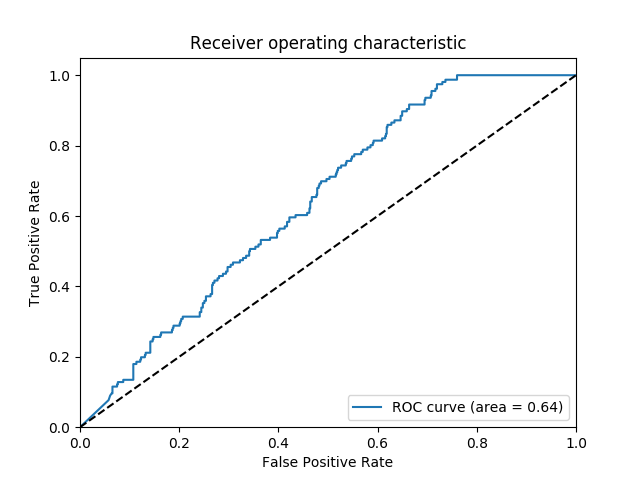
\includegraphics[width=12cm]{roc_01_00}
\caption{$\eta = 0.01$, $\mu=0.0$}
\end{figure}

\begin{figure}[!h]
\centering
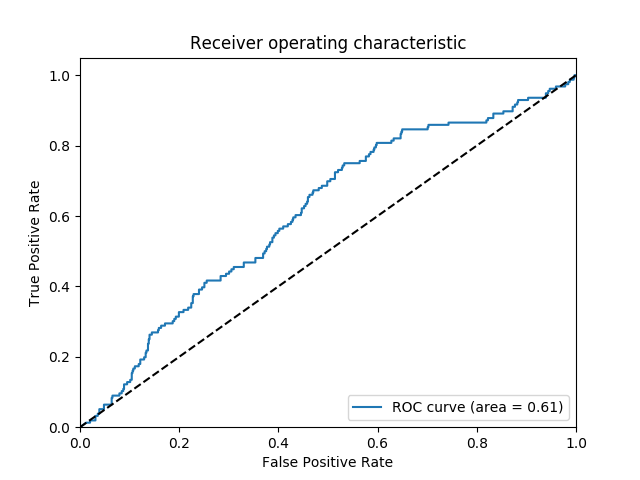
\includegraphics[width=12cm]{roc_10_10}
\caption{$\eta = 0.10$, $\mu=0.1$}
\end{figure}


\begin{figure}[!h]
\centering
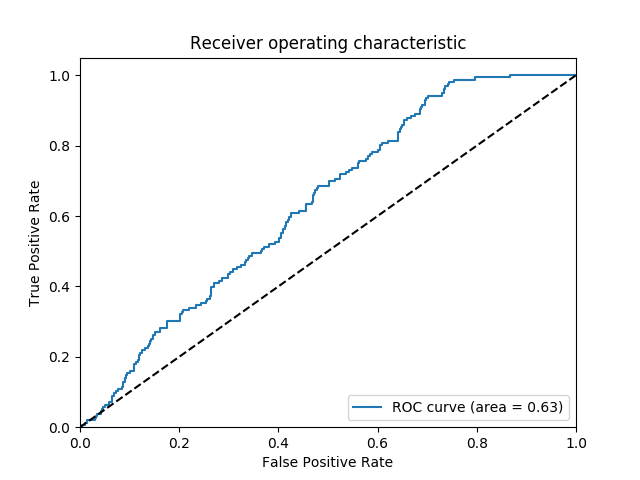
\includegraphics[width=12cm]{roc_01_90}
\caption{$\eta = 0.01$, $\mu=0.1$}
\end{figure}


\pagebreak

\subsection{Hadoop}
\textbf{c.} Compare the performance with that of previous problem and briefly analyze why the difference.

\vspace{5mm}
My ensemble learner performed very similar to the single learner, but it was
much less sensitive to an increase in learning rate, showing very little
decrease in ROC score as I increased $\eta$.  This is expected because we are
averaging across many results, which may have overshot the error minimum in
different directions.  These results are promising for big data problems,
because we can leverage tools like Hadoop to train many small models in parallel
and achieve similar results with an overall more robust model.


\end{document}
